\documentclass[jou,apacite, 10px]{apa6}
\usepackage{listings}
\usepackage{courier}
\usepackage{CJKutf8}
\usepackage[shortlabels]{enumitem}
\lstset{basicstyle=\small\ttfamily,breaklines=true}
\lstset{frame=single}
\makeatletter
\newcommand*{\rom}[1]{\expandafter\@slowromancap\romannumeral #1@}
\makeatother
\title{Classify a book's category based on its title}
\shorttitle{Book classification using book titles}

\twoauthors{Yunkai Wang}{Jules Kuehn}
\twoaffiliations{Carleton University, School of Computer Science}{Carleton University, School of Computer Science}

\abstract{Recently Convolutional Neural Networks (CNN) have been well-studied and be shown that they can archive incredible results on tasks like sentence classification (Kim, 2014; Zhang and Wallace, 2015). An interesting topic that has been studied is if we can categorize a book based on its cover picture (Iwana et al., 2016). "However, classification of books based on the cover image is a difficult task." (Iwana et al., 2016, p. 6). That being said, the relationship between the book's cover image and its category does exist, but it's hard to to classify using a CNN as many books have misleading cover images. Based on the idea of categorizing books, we are conducting this experiment to see if we can use CNN to learn the potential relationship between a books title and its categories. For this project, we will experiment how accurately this task can be performed with different model setups and layers (Britz, 2015) using matrixes that represent the titles as input (Mikolov et al., 2013; Karani, 2018; Britz, 2015).}

\leftheader{Wang, Kuehn}

\begin{document}
\maketitle    
                        
\section{\rom{1}. Introduction}
Book titles will given the reader a first impression of what the book may be about, and most of the time, a good book title will attract more readers from buying and reading the book, it makes the book different from other books (Peterson, 2018). But what does the book title really tells you? What can you say about the book by simply looking at the book title? If a title contains the word 'calendar', then most likely people will all agree that it's a calendar, but what if the book title doesn't contain a specific word that reveals its category, like if you are given the book title 'The Three-Body Problem' with knowing this book before, how will you categorize the book? Will the book title be sufficient for a CNN that has been pre-trained with titles and categories be able to detect that book as a science friction, or will the CNN think that it's a physics book? This is a very interesting question to ask, and that's why we conduct this experiment, to see if the computers are able to learn the potential relationship between a book's title and its category using CNN.

\section{\rom{2}. Background/Related work}

\subsection{Dateset}
The \textit{Data Mining} is a dataset that can be found on \textit{Github.com}, and it was published by the researchers who conducted the experiment on testing the relationship between a books cover image and its category (Iwana et al., 2016; uchidalab, 2018). The set consists of detailed information of $207572$ books from $32$ different categories. Some of the books are easy to classify, like 'calendar' and 'law', which are not similar to the other categories, or they contain some specific keyword among most books from the same category. However, many categories are similar, like 'Christian Books and Bibles' and 'Religion and Spirituality.'It is these categories that are the difficult part for the CNN to correctly classify. The dataset is not automatically splitted into training set and test set, so we use \textit{sklearn} library to split the data.

\subsection{Loading and transforming the data}
Here are the list of steps we took to load the dataset:

\rule{0pt}{4ex}  1. First we loaded all the original data line by line, and for each line, we extracted the books title and its category, as that was the only information we fed to our neural network.

\rule{0pt}{4ex}  2. Since most titles are of different length, and the maximum title length is $96$. We could expand the titles so that they all have length $96$. However, as Figure $1$ shows, most of titles have length less than $26$, only several titles have length $>26$. Therefore, we choose the maximum length to be $26$ instead of $96$. We used \textit{pad\_sequence} function from keras library to accomplish the task, which simply appends $0$ to the end of the titles that are shorter than the given length, and cut-off those long titles after $26$ words.

\begin{figure}[h!]
\captionsetup{justification=centering}
     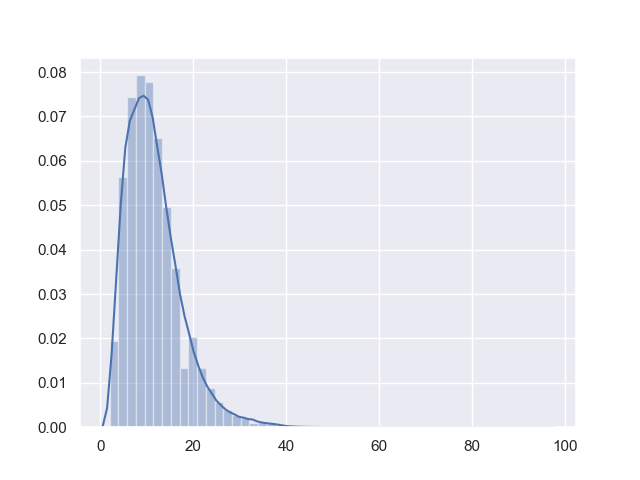
\includegraphics[width=0.5\textwidth]{images/title_lengths}
     \caption{Distributions of title lengths}
\end{figure}

\rule{0pt}{4ex}  3. With the help of \textit{train\_test\_split} function, we split the training data and testing data by having a testing data of size $10\%$ of the original dataset.

\rule{0pt}{4ex}  4. We convert the titles into matrices that can represent these titles, more details about this can be found in the 'Representing titles using matrices' section.

\subsection{Libraries}
In this project, we used the following libraries to avoid re-writing a lot of the codes that are not so important for the context of this experiment:

\begin{itemize}
\item keras: We used keras library a lot, like the data preprocessing functions and the functions that create the layers automatically.
\item sklearn: We used sklearn to split the training and testing dataset, and the TSNE function to plot the categories on a 2D graph.
\item tensorflow: Tensorflow was originally used in mlp.py and cnn.py files, and we used the models defined in those files to see how they perform on this task.
\end{itemize}

\subsection{Representing titles using matrices}
In order to apply CNNs to natural language processing (NLP) related tasks, the input are the words or sentences that are represented as matrices (Britz, 2015). Typically, we can use one of the two following mechanisms to represent the titles:
\begin{itemize}
\item Word embeddings: Using \textit{word2vec}("Word2vec", 2018) or \textit{GloVe}("GloVe: Global Vectors for Word Representation", 2014) to generate low-rank approximation of these titles (Karani, 2018).
\item One-hot: Convert the words into unique indices that represent these words, so each title becomes a vector of indices. This can be done using the \textit{one\_hot} function that is available in \textit{keras} library.
\end{itemize}

\section{\rom{3}. Problem Statement}

We want computers to be able to handle the categorization tasks for books based on book titles, such that in the future, the computer will be able to auto-categorize a new book given only its title, which will be faster than manually categorizing the books. It's almost impossible to manually design a rule-based program, that will handle the categorization problem nicely and accurately. The titles and the categories don't have an obvious relationship which we can use to linearly separate the titles into categories, there may be infinitely many potential relationships. However, if we success with our experiment, then we can use CNN to learn the underlying relationship between the titles and the categories, and the CNN will achieve a high accuracy in the categorization task.

\section{\rom{4}. Model}
We began with 2 naive implementations, in which each "word vector" was an arbitrary unique integer. Each title is then a vector of these integers (one for each word), zero padded to the length of the longest title (96 words). This representation of the titles has little semantic value as the integers representing the words are arbitrary.\\

% Insert diagram of naive model
The first naive model was a fully connected MLP with the following configuration. Output size of each layer is indicated in parentheses.

\begin{itemize}
    \item Input (96)
    \item FC Sigmoid (625)
    \item FC Sigmoid (300)
    \item FC Softmax (32)
\end{itemize}

The second naive model was based on a good model for the CIFAR-10 classification.

\begin{itemize}
    \item Input (96,1)
    \item Conv ReLU: 3 kernel, 1 stride (96,32)
    \item Conv ReLU: 3 kernel, 1 stride (96,32)
    \item Max pool: 2 kernel, 2 stride (48,32)
    \item Dropout: pKeep 0.8 (48,32)
    \item Conv ReLU: 3 kernel, 1 stride (48,64)
    \item Max pool: 2 kernel, 2 stride (24,64)
    \item Conv ReLU: 3 kernel, 1 stride (24,64)
    \item Max pool: 24 kernel, 24 stride (1,64)
    \item Dropout: pKeep 0.8 (1,64)
    \item Output Softmax (32)
\end{itemize}

A better word representation is to embed each word in a n-dimensional space, where the position of each word reflects its meaning in relation to the other words. Each word is then represented by a dense vector of length n, with similar words having similar vectors. Similarity between words is inferred from context. Many pre-trained embeddings are available, trained through Word2Vec or GloVe on datasets pulled from Wikipedia, Twitter, or other sources. An embedding can also be trained from scratch, or initialized to a pre-trained dataset then trained further. We compare these three approaches.\\

The first embedding model trained the embeddings from scratch, using only the book titles from the training set. Note that we truncated the titles from a maximum of 96 words to 26 words. We chose 32 for the embedding dimension, based on the rule of the thumb that the embedding should be the fourth root of the vocabulary size. There were roughly 70,000 words in the training dataset, which suggest that the embedding dimension should be 16, but we found that 32 offered a slight improvement in practice.
\begin{itemize}
    \item Input (26, 1)
    \item Embedding (26, 32)
    \item Flatten (832)
    \item Dropout 0.5 (832)
    \item Output Softmax (32)
\end{itemize}

The second embedding model loaded 400,000 pre-trained 100-dimensional word-vectors from the GloVe.6B dataset. These word vectors were trained on Wikipedia and Gigaword, a newswire dataset. The model is identical to EmbedTrain except that the embeddings are pre-trained and fixed, with the embedding dimension increased to 100.\\

The third embedding model is identical to EmbedTrain except that the embeddings are initialized to the GloVe dataset as seen in EmbedGloveFixed. Embeddings are then retrained on the book titles.\\

For each of the three embedding models, we also tested 2 variations to compare the performance of MLP vs CNN on the title embeddings. The first variation adds a single fully connected (FC) layer:

\begin{itemize}
    \item Input (26, 1)
    \item Embedding (26, 32)
    \item Flatten (832)
    \item \textbf{FC ReLU (512)}
    \item Dropout 0.5 (512)
    \item Output Softmax (32)
\end{itemize}

The second variation adds a single convolutional layer, followed by maxpool over the entire length:

\begin{itemize}
    \item Input (26, 1)
    \item Embedding (26, 32)
    \item \textbf{Conv ReLU: 3 kernel, 1 stride (24, 512)}
    \item \textbf{Max pool: 24 kernel, 24 stride (1, 512)}
    \item Flatten (512)
    \item Dropout 0.5 (512)
    \item Output Softmax (32)\\
\end{itemize}

\section{\rom{4}. Implementation}

The naive models were implemented using the course-provided cnn.py and mlp.py code. All other models were implemented in Keras, in which the code for the simple model is very concise:\\

\lstinputlisting{code/kerasModel.py}

\rule{0pt}{4ex} As training the models is computationally intensive, we ran many of our tests on Google Colaboratory.\\

\section{\rom{5}. Experiment}
Eleven distinct models were tested. Each model was tuned in terms of hyperparameters and dropout layers through experimentation, so they each represent a fair example of the architecture.\\

All models were run for at least 25 epochs, with a learning rate of 0.001, a batch size of 128, and an embedding length of 32 (except in the case of using the 100-dimensional GloVe embeddings). Of the 207572 labelled data, we took 9/10 for training and 1/10 for validation.\\

The results of the naive model, in which no meaning is embedded in the input vector, were predictably poor. The MLP achieved only 9\% validation accuracy, while the CNN eventually reached 12\%. While these accuracies are better than chance ($\approx$3\%), they are far from useful. There needs to be a meaningful representation of the input words in the input vectors, not arbitrary word indices.\\

Adding an embedding layer drastically improved the results. The best 7 models performed very similarly, all falling between 62 and 66\%.

\begin{figure}[h!]
\captionsetup{justification=centering}
    \centering
     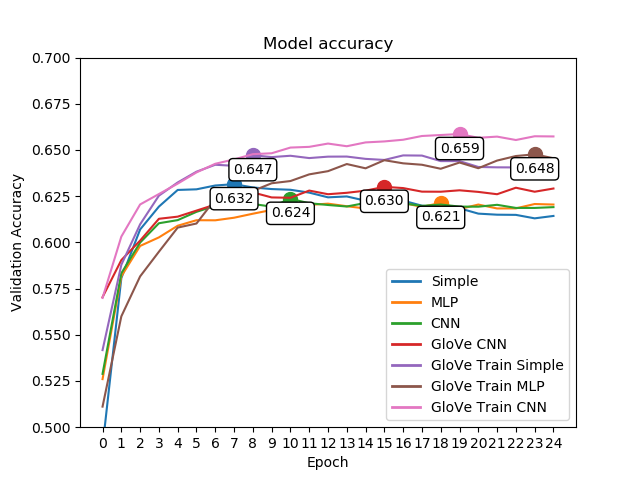
\includegraphics[width=0.5\textwidth]{images/good_models_comparison_small}
        \caption{Categorization accuracy for 7 best models}
\end{figure}

After training the model, we tested the dataset by category to get a prediction vector which represented the mean of the predictions for all titles in the validation set belonging to that category. Projecting these 32-dimensional means into 2 dimensions using T-SNE, we can see that meaningful spatial relationships between categories have emerged. For instance, fiction categories Literature, Romance, and Mystery are close to each other, but far away from personal growth categories like Parenting, Self-Help, and Fitness. These relationships can also be seen in the top 5 categorizations for titles in a given category (see Appendix).

\begin{figure}[h!]
\captionsetup{justification=centering}
    \centering
     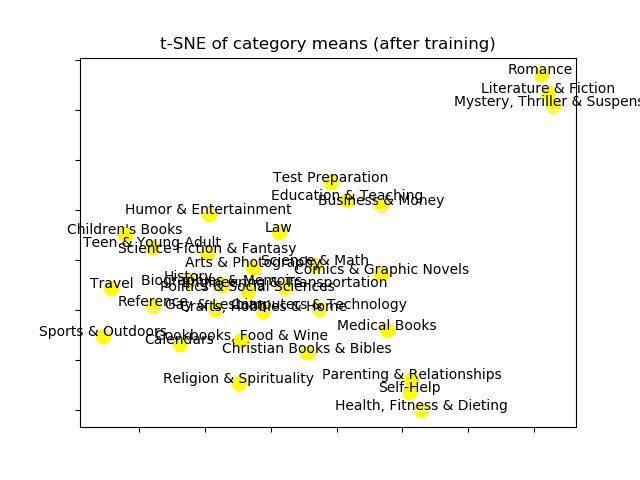
\includegraphics[width=0.5\textwidth]{images/tsne-categories-small}
        \caption{Spatial relationships between categories}
\end{figure}

\subsection{Training embeddings from dataset}
The simple model (code shown above) simply trained the embedding for the vocabulary of the book titles, creating relationships between individual word embeddings and the book categories in the process. The input word vectors, previously organized in rows (one vector per word) were then flattened into a single input vector for the title and fully connected to the 32 category softmax output. This worked very well (~80 to 90\% accuracy) in certain categories for which specific words consistently appeared, like Calendars.\\

Adding fully connected layers to create a multi-layer perceptron did not improve this model. The MLP variant was prone to overfitting, and was slower to propagate error correction through to the embedding layer.\\

The CNN model also didn't outperform the simple model. This suggests that the embedding layer, already taking advantage of word context and the labels of the specific dataset, is sufficient for the task.

\subsection{Using pre-trained GloVe embeddings}
The GloVe embeddings contain a vocabulary of 400,000 words. Since we disallowed training for this model, that meant words not found in the dataset would not be placed meaningfully in the embedding space. The missing words were set to the 0 vector. We did not explore whether the disclusion of rare words is a negative or positive for this problem, but this is the subject of other researchs in NLP. Out of the 75,094 words in the titles, 20,429 (27\%) were not found in GloVe dataset.\\

Performing experiments on the pre-trained GloVe embeddings better supported our hypothesis that a CNN would be a good choice for this problem. With the simple model (title matrices flattened and fully connected to the softmax output), there was insufficient trainable parameters (83,232) to fit the data to the labels, reaching a plateau at roughly 50\% accuracy on the validation data, and less than 60\% even on the training data.\\

\begin{figure}[h!]
\captionsetup{justification=centering}
    \centering
     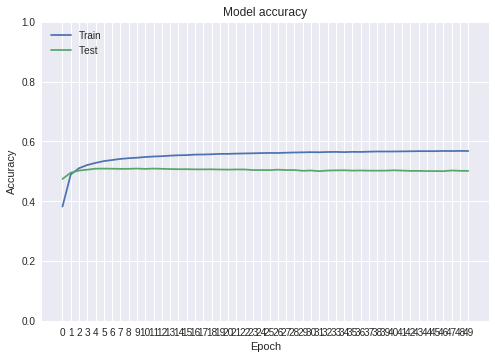
\includegraphics[width=0.5\textwidth]{images/Training-Glove}
        \caption{GloVe embeddings straight into softmax}
\end{figure}

The MLP model did little to improve validation accuracy, reaching 54\% after 14 epochs. While the millions of trainable parameters (3,204,640) improved training accuracy to 80\% at 50 epochs, the patterns it was learning were not generalizable.\\

\begin{figure}[h!]
\captionsetup{justification=centering}
    \centering
     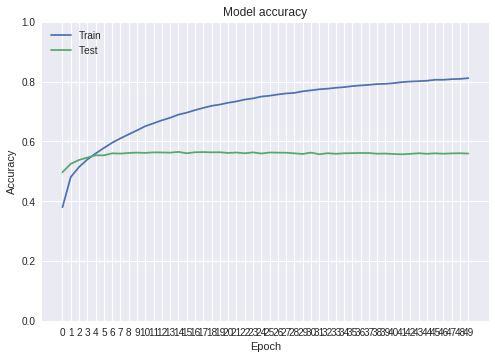
\includegraphics[width=0.5\textwidth]{images/Training-GloveMLP}
        \caption{GloVe embeddings through MLP}
\end{figure}

Adding the convolutional model suggested by Britz (2015a) improved the validation accuracy to the point of being competitive with the embeddings trained from the titles (63\%) while having a modest number of trainable parameters (433,184). This was the most convincing result in support of our hypothesis that the CNN would improve categorization accuracy. In contrast with the MLP above, the training clearly had better ability to generalize to unseen titles. This is not surprising, as the MLP would be considering the position of words in the title, whereas the CNN would be looking for words, or combinations of words, in any location in the title, disregarding precisely where in the title they appear. This property of spatial invariance is crucial for creating closer associations between individual word vectors and the category labels.

\subsection{Re-training GloVe embeddings from dataset}
In this model, we initialized our embeddings to the pre-trained GloVe set and then re-trained based on the titles and labels. Instead of initializing the missing words to zero, we initialized them randomly and allowed them to be trained along with the rest of the pre-trained embeddings. The three tested variations on this model performed the best of all tested models.\\

The simple model converged to a peak validation accuracy of 64.7\% in 9 epochs. The training accuracy continues to increase at 50 epochs, showing similarity to the MLP with non-trainable embeddings discussed previously. This makes sense, as this model also has a huge number of trainable parameters (7,592,632).\\

\begin{figure}[h!]
\captionsetup{justification=centering}
    \centering
     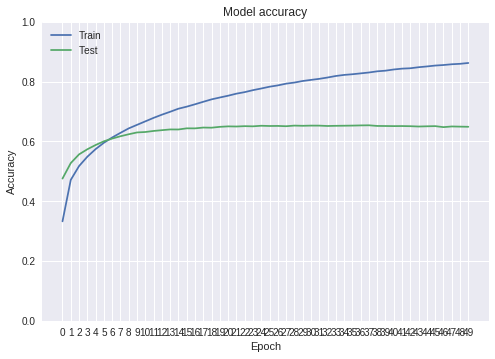
\includegraphics[width=0.5\textwidth]{images/Training-GloveTrainable}
        \caption{GloVe initialized but trainable}
\end{figure}

Adding fully connected layers didn't much improve on this result, reaching around the same accuracy (64.8\%) but taking 24 epochs to do so. As previously discussed, there are sufficient trainable parameters in the embedding to categorize the data - the addition of more parameters only slows down learning.\\

The CNN model performed the best of all tested models, with 66\% validation accuracy at 20 epochs, and the best accuracy at any epoch of any model. Since the filters can learn spatially invariant word associations with categories, the relationship between words and these categories does not need to be captured in the word embedding. Thus, the generalized semantic relationships of the words, captured in the GloVe training on a much larger dataset, is retained. Apart from the slow training on 7,942,584 parameters, this model is the most promising.\\

\subsection{Factors in the dataset affecting categorization accuracy}
Aside from the particular configuration of the models, certain factors in the dataset affected the accuracy. The most substantial were found to be title length and category. Titles of less than 5 words had noticeably worse accuracy, with one word titles being categorized correctly only 30\% of the time. However, accuracy did not substantially improve as the length increased over 5 words. (The figure was generated from the simple embedding model).\\

\begin{figure}[h!]
\captionsetup{justification=centering}
    \centering
        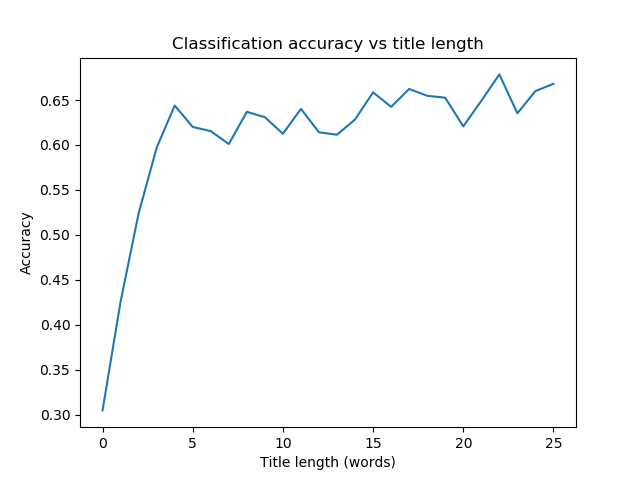
\includegraphics[width=0.5\textwidth]{images/title-length-accuracy-white}
        \caption{Classification accuracy is a function of length}
\end{figure}

The accuracy also varied by category. Based on manual inspection of the data, certain categories have distinct words which consistently appear in the titles (like "Calendar" or "Cookbook") which directly mirror the category. Other highly accurate categories like Computers, Medical, and Law often include domain-specific words in the titles. The worst performing categories (Biographies, Parenting, Politics, Self-Help) have more varied titles.\\

\begin{figure}[h!]
    \captionsetup{justification=centering}
        \centering
            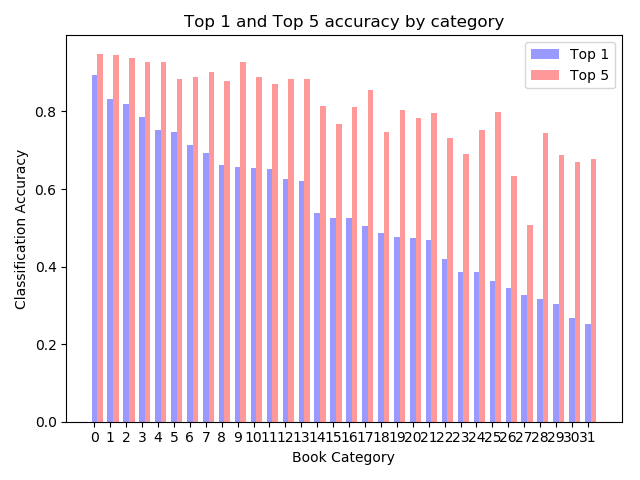
\includegraphics[width=0.5\textwidth]{images/Category_Top1_Top5}
            \caption{Certain categories achieve better accuracy}
    \end{figure}

Titles from certain categories also exhibit more overlap in terms of potential categorization. By looking at the T-SNE plot of category means, and the accompanying table of categorical output by categorical input, we can see that certain categories cluster closely together and have high error between them. The top 5 accuracy for these categories is still fairly good.\\
Finally, such a system could never achieve 100\% accuracy while there are errors or inconsistency in the training and test data. "Carrying off the Cherokee: History of Buffington's Company Georgia Mounted Militia", which the network categorized as History, was actually labelled "Crafts, Hobbies & Home". Other books do not fit cleanly into one category or another, such as "Indonesia (Country Explorers)", which the network categorized as Travel. The actual label was "Children's Books". This title demonstrates how a children's travel book would never achieve good categorization accuracy, since one could reasonably place it in either category.

\section{\rom{6}. Conclusion}
In this project, we experimented using different neural network models to categorize book based on its title, and we archived a better result compared with the accuracies if the neural network judge the book based on its cover image (Iwana et al.). We have shown that with word embedding and a very simple neural network model, we are able to categorize the books accurately, even though it's not categorizing well for some of the categories. However, since the neural network is very small, we are able to train the network within a reasonable short time, which makes it possible to train the network with a larger dataset in order to improve the result, especially feeding more training datas for those similar categories. For future improvement, we can try to make the CNN more complicated, or finding a new neural network model that is better at this job. but that will definitely make it harder to train the network with large data set because of the computational complexity. Another possibility to improve the result is to filter out some of the confusion words, or misleading words among the titles, where these words are the most common words that will cause a book title to be incorrectly categorized, but that's beyond the scope of this project as that requires a lot more data pre-processing and experiments on which set of words we should filter out in order to improve the result.\\

 The \textit{Data Mining} dataset is an interesting dataset to be working on, as it provides the capability to conducting many different possible classification experiments, like the relationship between a book title and the book author, etc. However, if the original dataset can provide a typical sentence from each book (like the first sentence from the book or the best sentence from the book), then we can conduct even more interesting experiments. Also, it will be helpful if people can enrich that dataset with more books that belong those small sized categories like Education \& training, which will definitely improve the classification accuracy of our model, and possibly the others.

\section{References}
\begin{enumerate}[(1)]
\item Britz, D. (2015a, November 7). Understanding Convolutional Neural Networks for NLP. Retrieved December 11, 2018, from http://www.wildml.com/2015/11/understanding-convolutional-neural-networks-for-nlp/
\item Britz, D. (2015b, December 11). Implementing a CNN for Text Classification in TensorFlow. Retrieved December 11, 2018, from http://www.wildml.com/2015/12/implementing-a-cnn-for-text-classification-in-tensorflow/
\item GloVe: Global Vectors for Word Representation. (n.d.). Retrieved December 15, 2018, from https://nlp.stanford.edu/projects/glove/
\item Iwana, B. K., Rizvi, S. T. R., Ahmed, S., Dengel, A., \& Uchida, S. (2016). Judging a Book By its Cover. ArXiv:1610.09204 [Cs]. Retrieved from http://arxiv.org/abs/1610.09204
\item Karani, D. (2018, September 1). Introduction to Word Embedding and Word2Vec. Retrieved December 11, 2018, from https://towardsdatascience.com/introduction-to-word-embedding-and-word2vec-652d0c2060fa
\item Kim, Y. (2014). Convolutional Neural Networks for Sentence Classification. ArXiv:1408.5882 [Cs]. Retrieved from http://arxiv.org/abs/1408.5882
Mikolov, T., Chen, K., Corrado, G., \& Dean, J. (2013). Efficient Estimation of Word Representations in Vector Space. ArXiv:1301.3781 [Cs]. Retrieved from http://arxiv.org/abs/1301.3781
\item Peterson, V. (n.d.). How to Write an Effective Book Title. Retrieved December 15, 2018, from https://www.thebalancecareers.com/how-to-write-a-book-title-insights-and-examples-2799918
\item This dataset contains 207,572 books from the Amazon.com, Inc. marketplace.: uchidalab/book-dataset. (2018). Python, \begin{CJK}{UTF8}{min}九州大学 ヒューマンインタフェース研究室\end{CJK}. Retrieved from https://github.com/uchidalab/book-dataset (Original work published 2017)
\item Word2vec. (2018). In Wikipedia. Retrieved from https://en.wikipedia.org/w/index.php?title=Word2vec\& oldid=869116438
\item Zhang, Y., \& Wallace, B. (2015). A Sensitivity Analysis of (and Practitioners’ Guide to) Convolutional Neural Networks for Sentence Classification. ArXiv:1510.03820 [Cs]. Retrieved from http://arxiv.org/abs/1510.03820
\item https://blog.keras.io/using-pre-trained-word-embeddings-in-a-keras-model.html
\end{enumerate}

\onecolumn

\section*{Appendix}
Additional results from our experiments are shown here. See \textbf{V. Experiment} for details and analysis.

\begin{figure}[h!]
    \captionsetup{justification=centering}
  \centering
    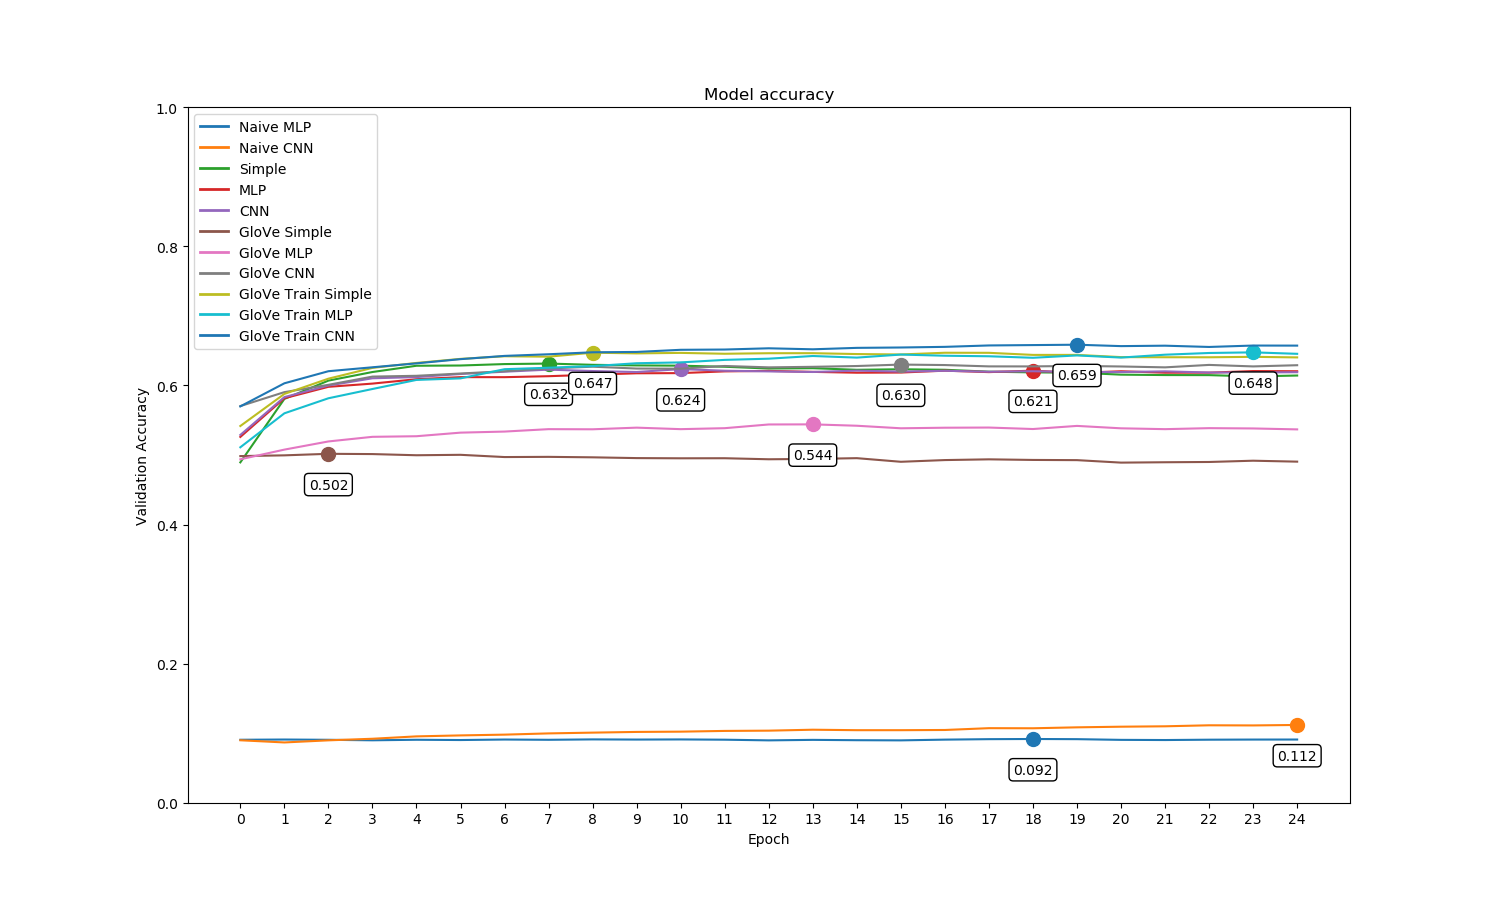
\includegraphics[width=0.9\columnwidth]{images/all_models_comparison}
  \caption{Validation accuracy for all 11 tested models}
    \label{all_models_comparison}
\end{figure}

\begin{figure}[h!]
    \captionsetup{justification=centering}
    \centering
    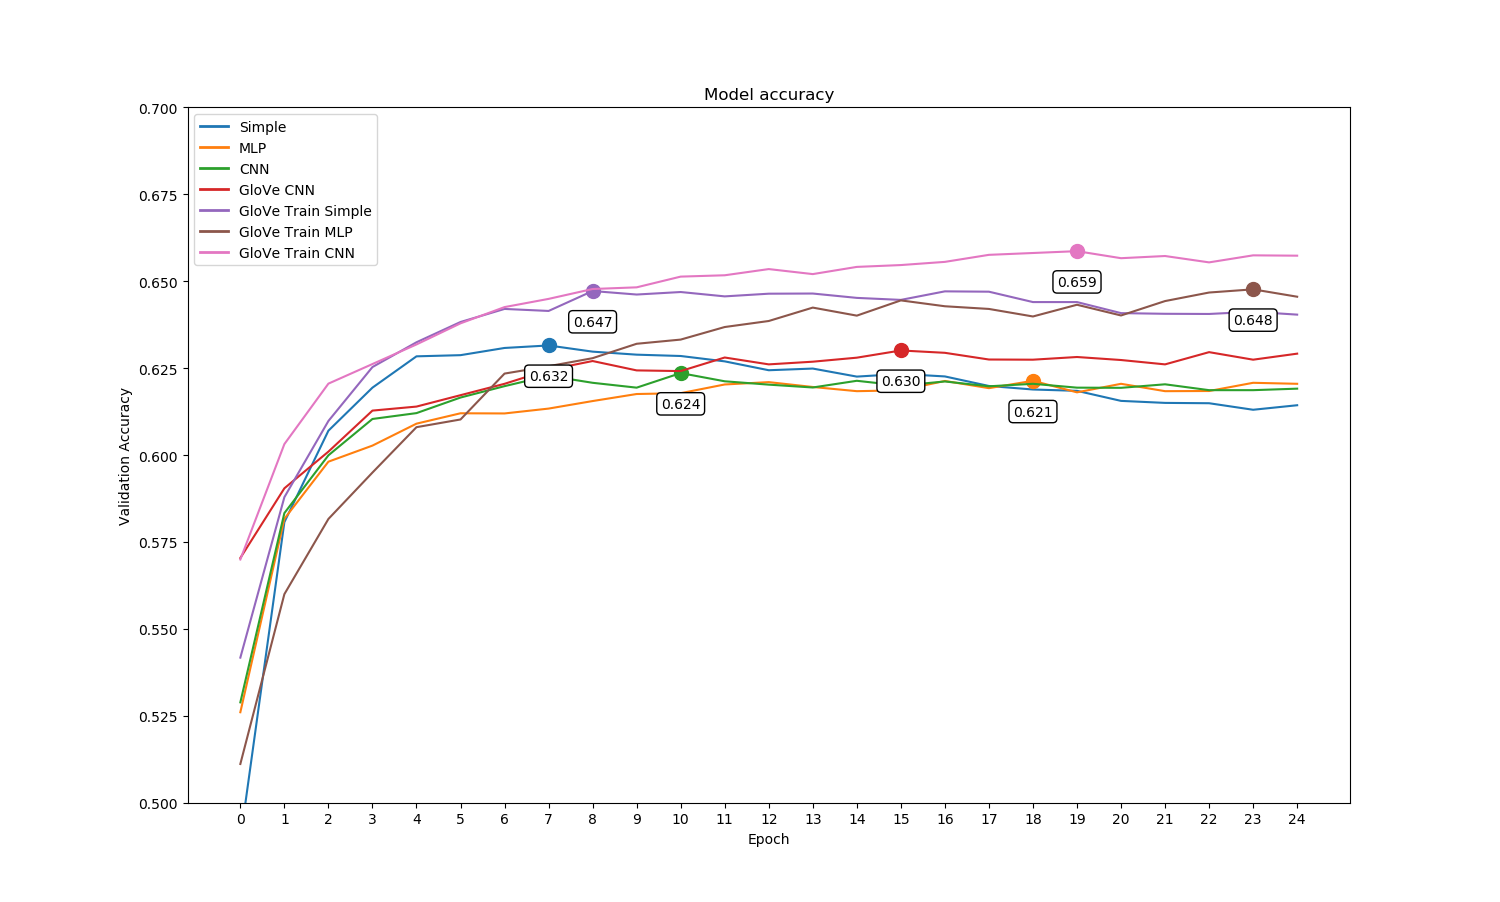
\includegraphics[width=0.9\columnwidth]{images/good_models_comparison}
    \caption{Validation accuracy for 7 best models (detail)}
    \label{good_models_comparison_small}
\end{figure}

\begin{figure}[h!]
    \captionsetup{justification=centering}
    \centering
      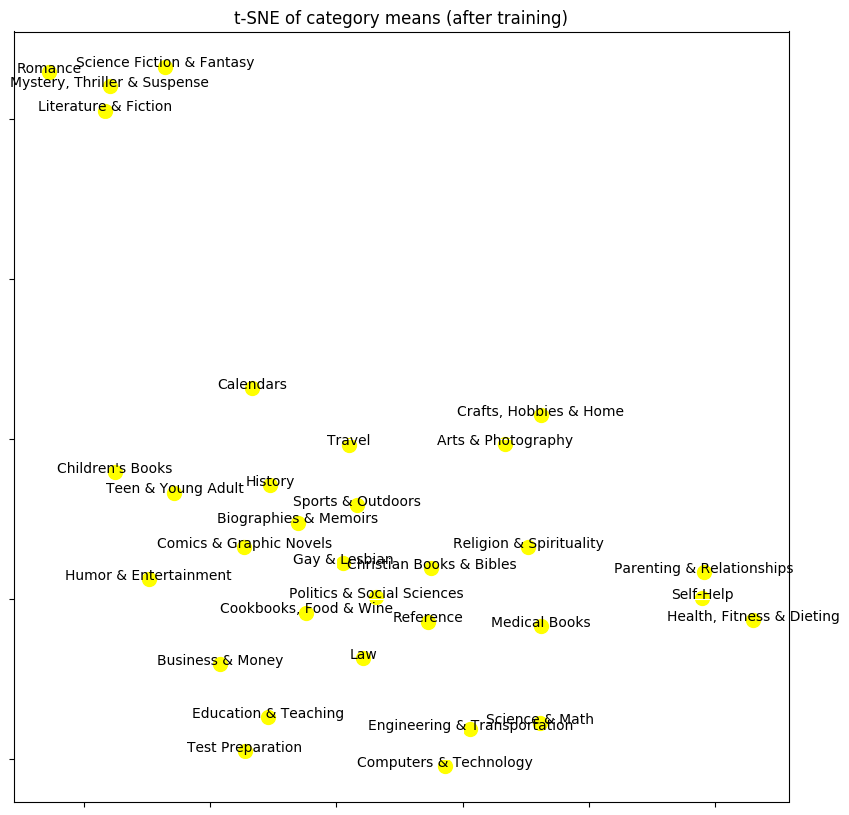
\includegraphics[width=\columnwidth]{images/tsne-categories}
    \caption{T-SNE projection of means of all validation titles by category}
      \label{tsne_categories}
  \end{figure}

% \twocolumn

% \begin{figure}[h!]
%     \captionsetup{justification=centering}
%         \centering
%          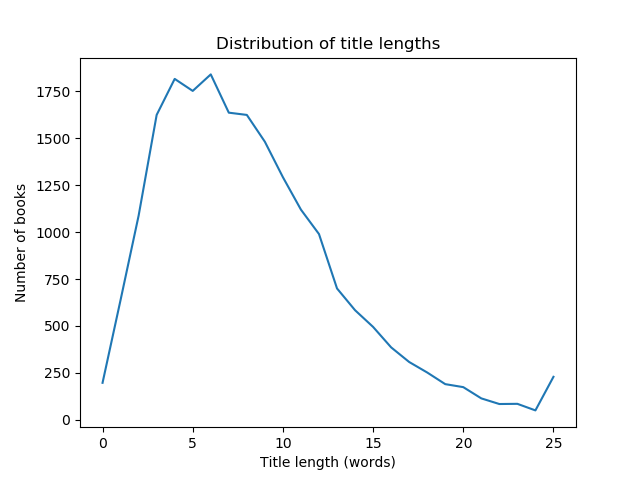
\includegraphics[width=0.5\textwidth]{images/title-lengths-white}
%             \caption{Length distribution of titles in validation set}
%     \end{figure}

\onecolumn

\begin{figure}[h!]
    \captionsetup{justification=centering}
        \centering
            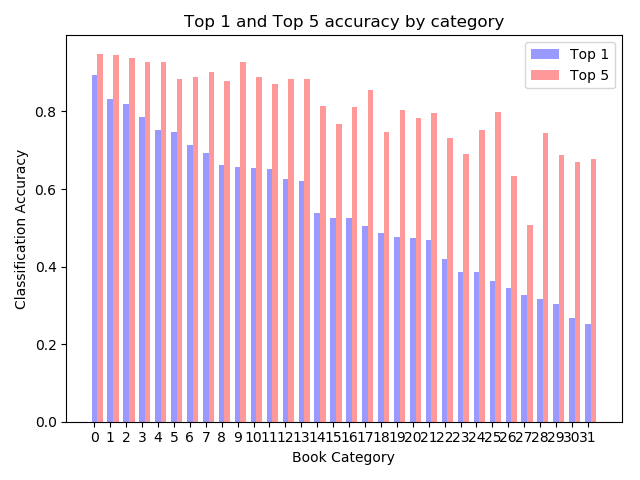
\includegraphics[width=0.5\textwidth]{images/Category_Top1_Top5}
            \caption{Certain categories achieve better accuracy}
    \end{figure}

\lstinputlisting{code/Category_Top1_Top5.txt}

\twocolumn

\lstinputlisting{code/Category_Predictions.txt}

\end{document}
